\begin{figure}[p]
  \caption[Confronto prestazioni delle due implementazioni dei canali]{Confronto della scalabilit\`a e del tempo di servizio tra le due implementazioni con tempo di interarrivo $\inTa = 4\cdot10^3 \, \tau = 4.6265 \, \microsec$}
  \begin{subfigure}[b]{.5\columnwidth}
    \centering
    \renewcommand\thesubfigure{\alph{subfigure}}
    %% se vuoi spostare questa caption in fondo devi modificare anche i contatori!
    \caption{Scalabilit\`a del tempo di servizio}
    \begin{subfigure}[b]{\textwidth}
      \centering
      \addtocounter{subfigure}{-1}
      \renewcommand\thesubfigure{\alph{subfigure}1}
      \resizebox{\columnwidth}{!}{% GNUPLOT: LaTeX picture with Postscript
\begingroup
  \makeatletter
  \providecommand\color[2][]{%
    \GenericError{(gnuplot) \space\space\space\@spaces}{%
      Package color not loaded in conjunction with
      terminal option `colourtext'%
    }{See the gnuplot documentation for explanation.%
    }{Either use 'blacktext' in gnuplot or load the package
      color.sty in LaTeX.}%
    \renewcommand\color[2][]{}%
  }%
  \providecommand\includegraphics[2][]{%
    \GenericError{(gnuplot) \space\space\space\@spaces}{%
      Package graphicx or graphics not loaded%
    }{See the gnuplot documentation for explanation.%
    }{The gnuplot epslatex terminal needs graphicx.sty or graphics.sty.}%
    \renewcommand\includegraphics[2][]{}%
  }%
  \providecommand\rotatebox[2]{#2}%
  \@ifundefined{ifGPcolor}{%
    \newif\ifGPcolor
    \GPcolortrue
  }{}%
  \@ifundefined{ifGPblacktext}{%
    \newif\ifGPblacktext
    \GPblacktexttrue
  }{}%
  % define a \g@addto@macro without @ in the name:
  \let\gplgaddtomacro\g@addto@macro
  % define empty templates for all commands taking text:
  \gdef\gplbacktext{}%
  \gdef\gplfronttext{}%
  \makeatother
  \ifGPblacktext
    % no textcolor at all
    \def\colorrgb#1{}%
    \def\colorgray#1{}%
  \else
    % gray or color?
    \ifGPcolor
      \def\colorrgb#1{\color[rgb]{#1}}%
      \def\colorgray#1{\color[gray]{#1}}%
      \expandafter\def\csname LTw\endcsname{\color{white}}%
      \expandafter\def\csname LTb\endcsname{\color{black}}%
      \expandafter\def\csname LTa\endcsname{\color{black}}%
      \expandafter\def\csname LT0\endcsname{\color[rgb]{1,0,0}}%
      \expandafter\def\csname LT1\endcsname{\color[rgb]{0,1,0}}%
      \expandafter\def\csname LT2\endcsname{\color[rgb]{0,0,1}}%
      \expandafter\def\csname LT3\endcsname{\color[rgb]{1,0,1}}%
      \expandafter\def\csname LT4\endcsname{\color[rgb]{0,1,1}}%
      \expandafter\def\csname LT5\endcsname{\color[rgb]{1,1,0}}%
      \expandafter\def\csname LT6\endcsname{\color[rgb]{0,0,0}}%
      \expandafter\def\csname LT7\endcsname{\color[rgb]{1,0.3,0}}%
      \expandafter\def\csname LT8\endcsname{\color[rgb]{0.5,0.5,0.5}}%
    \else
      % gray
      \def\colorrgb#1{\color{black}}%
      \def\colorgray#1{\color[gray]{#1}}%
      \expandafter\def\csname LTw\endcsname{\color{white}}%
      \expandafter\def\csname LTb\endcsname{\color{black}}%
      \expandafter\def\csname LTa\endcsname{\color{black}}%
      \expandafter\def\csname LT0\endcsname{\color{black}}%
      \expandafter\def\csname LT1\endcsname{\color{black}}%
      \expandafter\def\csname LT2\endcsname{\color{black}}%
      \expandafter\def\csname LT3\endcsname{\color{black}}%
      \expandafter\def\csname LT4\endcsname{\color{black}}%
      \expandafter\def\csname LT5\endcsname{\color{black}}%
      \expandafter\def\csname LT6\endcsname{\color{black}}%
      \expandafter\def\csname LT7\endcsname{\color{black}}%
      \expandafter\def\csname LT8\endcsname{\color{black}}%
    \fi
  \fi
  \setlength{\unitlength}{0.0500bp}%
  \begin{picture}(7200.00,5040.00)%
    \gplgaddtomacro\gplbacktext{%
      \csname LTb\endcsname%
      \put(814,1325){\makebox(0,0)[r]{\strut{} 10}}%
      \csname LTb\endcsname%
      \put(814,2015){\makebox(0,0)[r]{\strut{} 20}}%
      \csname LTb\endcsname%
      \put(814,2705){\makebox(0,0)[r]{\strut{} 30}}%
      \csname LTb\endcsname%
      \put(814,3395){\makebox(0,0)[r]{\strut{} 40}}%
      \csname LTb\endcsname%
      \put(814,4085){\makebox(0,0)[r]{\strut{} 50}}%
      \csname LTb\endcsname%
      \put(814,4775){\makebox(0,0)[r]{\strut{} 60}}%
      \csname LTb\endcsname%
      \put(1839,484){\makebox(0,0){\strut{} 10}}%
      \csname LTb\endcsname%
      \put(2832,484){\makebox(0,0){\strut{} 20}}%
      \csname LTb\endcsname%
      \put(3825,484){\makebox(0,0){\strut{} 30}}%
      \csname LTb\endcsname%
      \put(4818,484){\makebox(0,0){\strut{} 40}}%
      \csname LTb\endcsname%
      \put(5810,484){\makebox(0,0){\strut{} 50}}%
      \csname LTb\endcsname%
      \put(6803,484){\makebox(0,0){\strut{} 60}}%
      \put(176,2739){\rotatebox{-270}{\makebox(0,0){\strut{}scalability}}}%
      \put(3874,154){\makebox(0,0){\strut{}$n$ parallel degree}}%
    }%
    \gplgaddtomacro\gplfronttext{%
      \csname LTb\endcsname%
      \put(3322,4602){\makebox(0,0)[r]{\strut{}ideal scalability}}%
      \csname LTb\endcsname%
      \put(3322,4382){\makebox(0,0)[r]{\strut{}udn udn}}%
      \csname LTb\endcsname%
      \put(3322,4162){\makebox(0,0)[r]{\strut{}sm sm}}%
    }%
    \gplbacktext
    \put(0,0){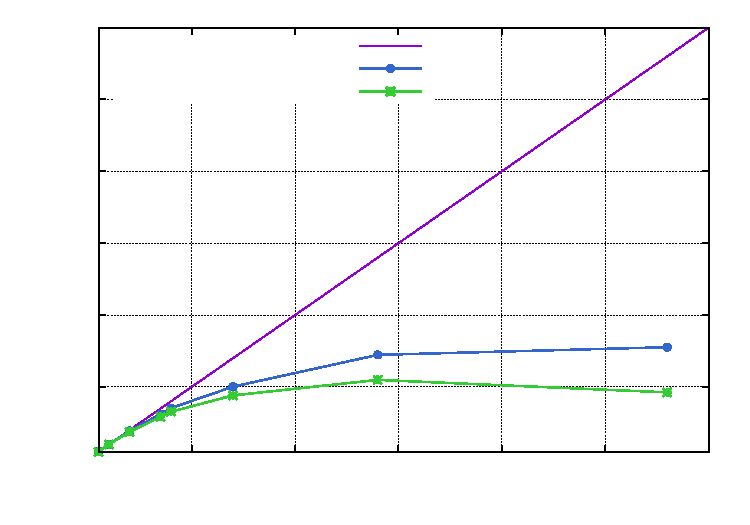
\includegraphics{plot-comp-T-s_nogatherInt_selected_500_4000_56}}%
    \gplfronttext
  \end{picture}%
\endgroup
}
      \caption{Dimensione della matrice 56x56}
      \label{fig:compare_s_udn_56}
    \end{subfigure}
    ~
    \begin{subfigure}[b]{\textwidth}
      \centering
      \addtocounter{subfigure}{-1}
      \renewcommand\thesubfigure{\alph{subfigure}2}
      \resizebox{\columnwidth}{!}{% GNUPLOT: LaTeX picture with Postscript
\begingroup
  \makeatletter
  \providecommand\color[2][]{%
    \GenericError{(gnuplot) \space\space\space\@spaces}{%
      Package color not loaded in conjunction with
      terminal option `colourtext'%
    }{See the gnuplot documentation for explanation.%
    }{Either use 'blacktext' in gnuplot or load the package
      color.sty in LaTeX.}%
    \renewcommand\color[2][]{}%
  }%
  \providecommand\includegraphics[2][]{%
    \GenericError{(gnuplot) \space\space\space\@spaces}{%
      Package graphicx or graphics not loaded%
    }{See the gnuplot documentation for explanation.%
    }{The gnuplot epslatex terminal needs graphicx.sty or graphics.sty.}%
    \renewcommand\includegraphics[2][]{}%
  }%
  \providecommand\rotatebox[2]{#2}%
  \@ifundefined{ifGPcolor}{%
    \newif\ifGPcolor
    \GPcolortrue
  }{}%
  \@ifundefined{ifGPblacktext}{%
    \newif\ifGPblacktext
    \GPblacktexttrue
  }{}%
  % define a \g@addto@macro without @ in the name:
  \let\gplgaddtomacro\g@addto@macro
  % define empty templates for all commands taking text:
  \gdef\gplbacktext{}%
  \gdef\gplfronttext{}%
  \makeatother
  \ifGPblacktext
    % no textcolor at all
    \def\colorrgb#1{}%
    \def\colorgray#1{}%
  \else
    % gray or color?
    \ifGPcolor
      \def\colorrgb#1{\color[rgb]{#1}}%
      \def\colorgray#1{\color[gray]{#1}}%
      \expandafter\def\csname LTw\endcsname{\color{white}}%
      \expandafter\def\csname LTb\endcsname{\color{black}}%
      \expandafter\def\csname LTa\endcsname{\color{black}}%
      \expandafter\def\csname LT0\endcsname{\color[rgb]{1,0,0}}%
      \expandafter\def\csname LT1\endcsname{\color[rgb]{0,1,0}}%
      \expandafter\def\csname LT2\endcsname{\color[rgb]{0,0,1}}%
      \expandafter\def\csname LT3\endcsname{\color[rgb]{1,0,1}}%
      \expandafter\def\csname LT4\endcsname{\color[rgb]{0,1,1}}%
      \expandafter\def\csname LT5\endcsname{\color[rgb]{1,1,0}}%
      \expandafter\def\csname LT6\endcsname{\color[rgb]{0,0,0}}%
      \expandafter\def\csname LT7\endcsname{\color[rgb]{1,0.3,0}}%
      \expandafter\def\csname LT8\endcsname{\color[rgb]{0.5,0.5,0.5}}%
    \else
      % gray
      \def\colorrgb#1{\color{black}}%
      \def\colorgray#1{\color[gray]{#1}}%
      \expandafter\def\csname LTw\endcsname{\color{white}}%
      \expandafter\def\csname LTb\endcsname{\color{black}}%
      \expandafter\def\csname LTa\endcsname{\color{black}}%
      \expandafter\def\csname LT0\endcsname{\color{black}}%
      \expandafter\def\csname LT1\endcsname{\color{black}}%
      \expandafter\def\csname LT2\endcsname{\color{black}}%
      \expandafter\def\csname LT3\endcsname{\color{black}}%
      \expandafter\def\csname LT4\endcsname{\color{black}}%
      \expandafter\def\csname LT5\endcsname{\color{black}}%
      \expandafter\def\csname LT6\endcsname{\color{black}}%
      \expandafter\def\csname LT7\endcsname{\color{black}}%
      \expandafter\def\csname LT8\endcsname{\color{black}}%
    \fi
  \fi
  \setlength{\unitlength}{0.0500bp}%
  \begin{picture}(7200.00,5040.00)%
    \gplgaddtomacro\gplbacktext{%
      \csname LTb\endcsname%
      \put(814,1325){\makebox(0,0)[r]{\strut{} 10}}%
      \csname LTb\endcsname%
      \put(814,2015){\makebox(0,0)[r]{\strut{} 20}}%
      \csname LTb\endcsname%
      \put(814,2705){\makebox(0,0)[r]{\strut{} 30}}%
      \csname LTb\endcsname%
      \put(814,3395){\makebox(0,0)[r]{\strut{} 40}}%
      \csname LTb\endcsname%
      \put(814,4085){\makebox(0,0)[r]{\strut{} 50}}%
      \csname LTb\endcsname%
      \put(814,4775){\makebox(0,0)[r]{\strut{} 60}}%
      \csname LTb\endcsname%
      \put(1839,484){\makebox(0,0){\strut{} 10}}%
      \csname LTb\endcsname%
      \put(2832,484){\makebox(0,0){\strut{} 20}}%
      \csname LTb\endcsname%
      \put(3825,484){\makebox(0,0){\strut{} 30}}%
      \csname LTb\endcsname%
      \put(4818,484){\makebox(0,0){\strut{} 40}}%
      \csname LTb\endcsname%
      \put(5810,484){\makebox(0,0){\strut{} 50}}%
      \csname LTb\endcsname%
      \put(6803,484){\makebox(0,0){\strut{} 60}}%
      \put(176,2739){\rotatebox{-270}{\makebox(0,0){\strut{}scalability}}}%
      \put(3874,154){\makebox(0,0){\strut{}$n$ parallel degree}}%
    }%
    \gplgaddtomacro\gplfronttext{%
      \csname LTb\endcsname%
      \put(3322,4602){\makebox(0,0)[r]{\strut{}ideal scalability}}%
      \csname LTb\endcsname%
      \put(3322,4382){\makebox(0,0)[r]{\strut{}udn udn}}%
      \csname LTb\endcsname%
      \put(3322,4162){\makebox(0,0)[r]{\strut{}sm sm}}%
    }%
    \gplbacktext
    \put(0,0){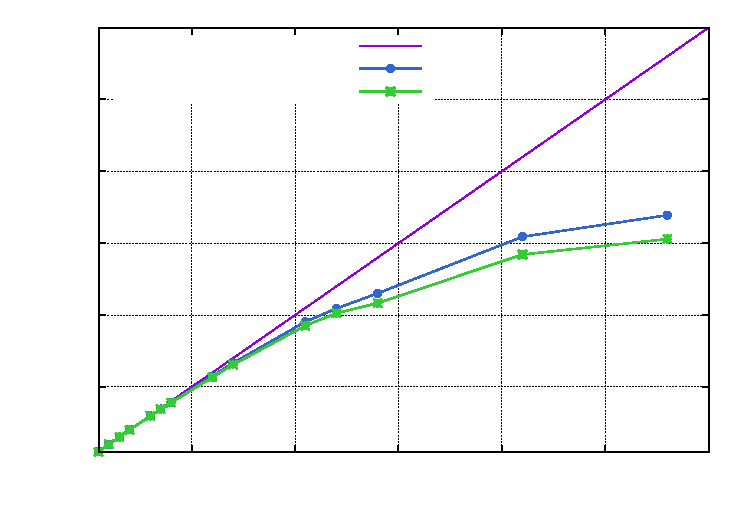
\includegraphics{plot-comp-T-s_nogatherInt_selected_500_20000_168}}%
    \gplfronttext
  \end{picture}%
\endgroup
}
      \caption{Dimensione della matrice 168x168}
      \label{fig:compare_s_udn_168}
    \end{subfigure}
    ~
    \begin{subfigure}[b]{\textwidth}
      \centering
      \addtocounter{subfigure}{-1}
      \renewcommand\thesubfigure{\alph{subfigure}3}
      \resizebox{\columnwidth}{!}{% GNUPLOT: LaTeX picture with Postscript
\begingroup
  \makeatletter
  \providecommand\color[2][]{%
    \GenericError{(gnuplot) \space\space\space\@spaces}{%
      Package color not loaded in conjunction with
      terminal option `colourtext'%
    }{See the gnuplot documentation for explanation.%
    }{Either use 'blacktext' in gnuplot or load the package
      color.sty in LaTeX.}%
    \renewcommand\color[2][]{}%
  }%
  \providecommand\includegraphics[2][]{%
    \GenericError{(gnuplot) \space\space\space\@spaces}{%
      Package graphicx or graphics not loaded%
    }{See the gnuplot documentation for explanation.%
    }{The gnuplot epslatex terminal needs graphicx.sty or graphics.sty.}%
    \renewcommand\includegraphics[2][]{}%
  }%
  \providecommand\rotatebox[2]{#2}%
  \@ifundefined{ifGPcolor}{%
    \newif\ifGPcolor
    \GPcolortrue
  }{}%
  \@ifundefined{ifGPblacktext}{%
    \newif\ifGPblacktext
    \GPblacktexttrue
  }{}%
  % define a \g@addto@macro without @ in the name:
  \let\gplgaddtomacro\g@addto@macro
  % define empty templates for all commands taking text:
  \gdef\gplbacktext{}%
  \gdef\gplfronttext{}%
  \makeatother
  \ifGPblacktext
    % no textcolor at all
    \def\colorrgb#1{}%
    \def\colorgray#1{}%
  \else
    % gray or color?
    \ifGPcolor
      \def\colorrgb#1{\color[rgb]{#1}}%
      \def\colorgray#1{\color[gray]{#1}}%
      \expandafter\def\csname LTw\endcsname{\color{white}}%
      \expandafter\def\csname LTb\endcsname{\color{black}}%
      \expandafter\def\csname LTa\endcsname{\color{black}}%
      \expandafter\def\csname LT0\endcsname{\color[rgb]{1,0,0}}%
      \expandafter\def\csname LT1\endcsname{\color[rgb]{0,1,0}}%
      \expandafter\def\csname LT2\endcsname{\color[rgb]{0,0,1}}%
      \expandafter\def\csname LT3\endcsname{\color[rgb]{1,0,1}}%
      \expandafter\def\csname LT4\endcsname{\color[rgb]{0,1,1}}%
      \expandafter\def\csname LT5\endcsname{\color[rgb]{1,1,0}}%
      \expandafter\def\csname LT6\endcsname{\color[rgb]{0,0,0}}%
      \expandafter\def\csname LT7\endcsname{\color[rgb]{1,0.3,0}}%
      \expandafter\def\csname LT8\endcsname{\color[rgb]{0.5,0.5,0.5}}%
    \else
      % gray
      \def\colorrgb#1{\color{black}}%
      \def\colorgray#1{\color[gray]{#1}}%
      \expandafter\def\csname LTw\endcsname{\color{white}}%
      \expandafter\def\csname LTb\endcsname{\color{black}}%
      \expandafter\def\csname LTa\endcsname{\color{black}}%
      \expandafter\def\csname LT0\endcsname{\color{black}}%
      \expandafter\def\csname LT1\endcsname{\color{black}}%
      \expandafter\def\csname LT2\endcsname{\color{black}}%
      \expandafter\def\csname LT3\endcsname{\color{black}}%
      \expandafter\def\csname LT4\endcsname{\color{black}}%
      \expandafter\def\csname LT5\endcsname{\color{black}}%
      \expandafter\def\csname LT6\endcsname{\color{black}}%
      \expandafter\def\csname LT7\endcsname{\color{black}}%
      \expandafter\def\csname LT8\endcsname{\color{black}}%
    \fi
  \fi
  \setlength{\unitlength}{0.0500bp}%
  \begin{picture}(7200.00,5040.00)%
    \gplgaddtomacro\gplbacktext{%
      \csname LTb\endcsname%
      \put(814,1325){\makebox(0,0)[r]{\strut{} 10}}%
      \csname LTb\endcsname%
      \put(814,2015){\makebox(0,0)[r]{\strut{} 20}}%
      \csname LTb\endcsname%
      \put(814,2705){\makebox(0,0)[r]{\strut{} 30}}%
      \csname LTb\endcsname%
      \put(814,3395){\makebox(0,0)[r]{\strut{} 40}}%
      \csname LTb\endcsname%
      \put(814,4085){\makebox(0,0)[r]{\strut{} 50}}%
      \csname LTb\endcsname%
      \put(814,4775){\makebox(0,0)[r]{\strut{} 60}}%
      \csname LTb\endcsname%
      \put(1839,484){\makebox(0,0){\strut{} 10}}%
      \csname LTb\endcsname%
      \put(2832,484){\makebox(0,0){\strut{} 20}}%
      \csname LTb\endcsname%
      \put(3825,484){\makebox(0,0){\strut{} 30}}%
      \csname LTb\endcsname%
      \put(4818,484){\makebox(0,0){\strut{} 40}}%
      \csname LTb\endcsname%
      \put(5810,484){\makebox(0,0){\strut{} 50}}%
      \csname LTb\endcsname%
      \put(6803,484){\makebox(0,0){\strut{} 60}}%
      \put(176,2739){\rotatebox{-270}{\makebox(0,0){\strut{}scalability}}}%
      \put(3874,154){\makebox(0,0){\strut{}$n$ parallel degree}}%
    }%
    \gplgaddtomacro\gplfronttext{%
      \csname LTb\endcsname%
      \put(3322,4602){\makebox(0,0)[r]{\strut{}ideal scalability}}%
      \csname LTb\endcsname%
      \put(3322,4382){\makebox(0,0)[r]{\strut{}udn udn}}%
      \csname LTb\endcsname%
      \put(3322,4162){\makebox(0,0)[r]{\strut{}sm sm}}%
    }%
    \gplbacktext
    \put(0,0){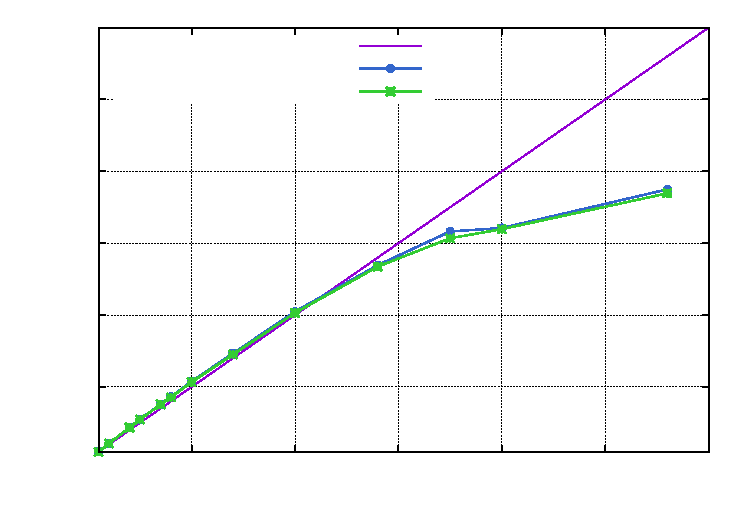
\includegraphics{plot-comp-T-s_nogatherInt_selected_500_50000_280}}%
    \gplfronttext
  \end{picture}%
\endgroup
}
      \caption{Dimensione della matrice 280x280}
      \label{fig:compare_s_udn_280}
    \end{subfigure}
    \label{fig:compare_s_udn}
  \end{subfigure}
  %%%%%%%%%%%%%%%%%%%%%%%%%%%%%%
  \hspace{2ex}
  %%%%%%%%%%%%%%%%%%%%%%%%%%%%%%
  \begin{subfigure}[b]{.5\columnwidth}
    \centering
    \renewcommand\thesubfigure{\alph{subfigure}}
    \caption{Tempi di servizio}
    \begin{subfigure}[b]{\textwidth}
      \centering
      \addtocounter{subfigure}{-1}
      \renewcommand\thesubfigure{\alph{subfigure}1}
      \resizebox{\columnwidth}{!}{% GNUPLOT: LaTeX picture with Postscript
\begingroup
  \makeatletter
  \providecommand\color[2][]{%
    \GenericError{(gnuplot) \space\space\space\@spaces}{%
      Package color not loaded in conjunction with
      terminal option `colourtext'%
    }{See the gnuplot documentation for explanation.%
    }{Either use 'blacktext' in gnuplot or load the package
      color.sty in LaTeX.}%
    \renewcommand\color[2][]{}%
  }%
  \providecommand\includegraphics[2][]{%
    \GenericError{(gnuplot) \space\space\space\@spaces}{%
      Package graphicx or graphics not loaded%
    }{See the gnuplot documentation for explanation.%
    }{The gnuplot epslatex terminal needs graphicx.sty or graphics.sty.}%
    \renewcommand\includegraphics[2][]{}%
  }%
  \providecommand\rotatebox[2]{#2}%
  \@ifundefined{ifGPcolor}{%
    \newif\ifGPcolor
    \GPcolortrue
  }{}%
  \@ifundefined{ifGPblacktext}{%
    \newif\ifGPblacktext
    \GPblacktexttrue
  }{}%
  % define a \g@addto@macro without @ in the name:
  \let\gplgaddtomacro\g@addto@macro
  % define empty templates for all commands taking text:
  \gdef\gplbacktext{}%
  \gdef\gplfronttext{}%
  \makeatother
  \ifGPblacktext
    % no textcolor at all
    \def\colorrgb#1{}%
    \def\colorgray#1{}%
  \else
    % gray or color?
    \ifGPcolor
      \def\colorrgb#1{\color[rgb]{#1}}%
      \def\colorgray#1{\color[gray]{#1}}%
      \expandafter\def\csname LTw\endcsname{\color{white}}%
      \expandafter\def\csname LTb\endcsname{\color{black}}%
      \expandafter\def\csname LTa\endcsname{\color{black}}%
      \expandafter\def\csname LT0\endcsname{\color[rgb]{1,0,0}}%
      \expandafter\def\csname LT1\endcsname{\color[rgb]{0,1,0}}%
      \expandafter\def\csname LT2\endcsname{\color[rgb]{0,0,1}}%
      \expandafter\def\csname LT3\endcsname{\color[rgb]{1,0,1}}%
      \expandafter\def\csname LT4\endcsname{\color[rgb]{0,1,1}}%
      \expandafter\def\csname LT5\endcsname{\color[rgb]{1,1,0}}%
      \expandafter\def\csname LT6\endcsname{\color[rgb]{0,0,0}}%
      \expandafter\def\csname LT7\endcsname{\color[rgb]{1,0.3,0}}%
      \expandafter\def\csname LT8\endcsname{\color[rgb]{0.5,0.5,0.5}}%
    \else
      % gray
      \def\colorrgb#1{\color{black}}%
      \def\colorgray#1{\color[gray]{#1}}%
      \expandafter\def\csname LTw\endcsname{\color{white}}%
      \expandafter\def\csname LTb\endcsname{\color{black}}%
      \expandafter\def\csname LTa\endcsname{\color{black}}%
      \expandafter\def\csname LT0\endcsname{\color{black}}%
      \expandafter\def\csname LT1\endcsname{\color{black}}%
      \expandafter\def\csname LT2\endcsname{\color{black}}%
      \expandafter\def\csname LT3\endcsname{\color{black}}%
      \expandafter\def\csname LT4\endcsname{\color{black}}%
      \expandafter\def\csname LT5\endcsname{\color{black}}%
      \expandafter\def\csname LT6\endcsname{\color{black}}%
      \expandafter\def\csname LT7\endcsname{\color{black}}%
      \expandafter\def\csname LT8\endcsname{\color{black}}%
    \fi
  \fi
  \setlength{\unitlength}{0.0500bp}%
  \begin{picture}(7200.00,5040.00)%
    \gplgaddtomacro\gplbacktext{%
      \csname LTb\endcsname%
      \put(946,704){\makebox(0,0)[r]{\strut{} 1}}%
      \csname LTb\endcsname%
      \put(946,2740){\makebox(0,0)[r]{\strut{} 10}}%
      \csname LTb\endcsname%
      \put(946,4775){\makebox(0,0)[r]{\strut{} 100}}%
      \csname LTb\endcsname%
      \put(1951,484){\makebox(0,0){\strut{} 10}}%
      \csname LTb\endcsname%
      \put(2922,484){\makebox(0,0){\strut{} 20}}%
      \csname LTb\endcsname%
      \put(3892,484){\makebox(0,0){\strut{} 30}}%
      \csname LTb\endcsname%
      \put(4862,484){\makebox(0,0){\strut{} 40}}%
      \csname LTb\endcsname%
      \put(5833,484){\makebox(0,0){\strut{} 50}}%
      \csname LTb\endcsname%
      \put(6803,484){\makebox(0,0){\strut{} 60}}%
      \put(176,2739){\rotatebox{-270}{\makebox(0,0){\strut{}service time ($\,\mu\mathrm{sec}$\,)}}}%
      \put(3940,154){\makebox(0,0){\strut{}$n$ parallel degree}}%
    }%
    \gplgaddtomacro\gplfronttext{%
      \csname LTb\endcsname%
      \put(3586,4602){\makebox(0,0)[r]{\strut{}ideal service time}}%
      \csname LTb\endcsname%
      \put(3586,4382){\makebox(0,0)[r]{\strut{}udn udn}}%
      \csname LTb\endcsname%
      \put(3586,4162){\makebox(0,0)[r]{\strut{}sm sm}}%
    }%
    \gplbacktext
    \put(0,0){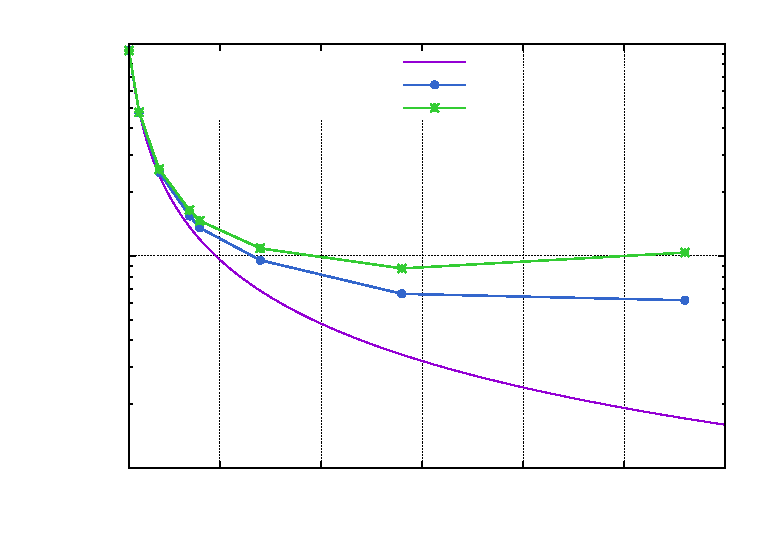
\includegraphics{plot-T-UDN-SM_nogatherInt_selected_500_selected_56}}%
    \gplfronttext
  \end{picture}%
\endgroup
}
      \caption{Dimensione della matrice 56x56}
      \label{fig:compare_s_sm_56}
    \end{subfigure}
    ~
    \begin{subfigure}[b]{\textwidth}
      \centering
      \addtocounter{subfigure}{-1}
      \renewcommand\thesubfigure{\alph{subfigure}2}
      \resizebox{\columnwidth}{!}{% GNUPLOT: LaTeX picture with Postscript
\begingroup
  \makeatletter
  \providecommand\color[2][]{%
    \GenericError{(gnuplot) \space\space\space\@spaces}{%
      Package color not loaded in conjunction with
      terminal option `colourtext'%
    }{See the gnuplot documentation for explanation.%
    }{Either use 'blacktext' in gnuplot or load the package
      color.sty in LaTeX.}%
    \renewcommand\color[2][]{}%
  }%
  \providecommand\includegraphics[2][]{%
    \GenericError{(gnuplot) \space\space\space\@spaces}{%
      Package graphicx or graphics not loaded%
    }{See the gnuplot documentation for explanation.%
    }{The gnuplot epslatex terminal needs graphicx.sty or graphics.sty.}%
    \renewcommand\includegraphics[2][]{}%
  }%
  \providecommand\rotatebox[2]{#2}%
  \@ifundefined{ifGPcolor}{%
    \newif\ifGPcolor
    \GPcolortrue
  }{}%
  \@ifundefined{ifGPblacktext}{%
    \newif\ifGPblacktext
    \GPblacktexttrue
  }{}%
  % define a \g@addto@macro without @ in the name:
  \let\gplgaddtomacro\g@addto@macro
  % define empty templates for all commands taking text:
  \gdef\gplbacktext{}%
  \gdef\gplfronttext{}%
  \makeatother
  \ifGPblacktext
    % no textcolor at all
    \def\colorrgb#1{}%
    \def\colorgray#1{}%
  \else
    % gray or color?
    \ifGPcolor
      \def\colorrgb#1{\color[rgb]{#1}}%
      \def\colorgray#1{\color[gray]{#1}}%
      \expandafter\def\csname LTw\endcsname{\color{white}}%
      \expandafter\def\csname LTb\endcsname{\color{black}}%
      \expandafter\def\csname LTa\endcsname{\color{black}}%
      \expandafter\def\csname LT0\endcsname{\color[rgb]{1,0,0}}%
      \expandafter\def\csname LT1\endcsname{\color[rgb]{0,1,0}}%
      \expandafter\def\csname LT2\endcsname{\color[rgb]{0,0,1}}%
      \expandafter\def\csname LT3\endcsname{\color[rgb]{1,0,1}}%
      \expandafter\def\csname LT4\endcsname{\color[rgb]{0,1,1}}%
      \expandafter\def\csname LT5\endcsname{\color[rgb]{1,1,0}}%
      \expandafter\def\csname LT6\endcsname{\color[rgb]{0,0,0}}%
      \expandafter\def\csname LT7\endcsname{\color[rgb]{1,0.3,0}}%
      \expandafter\def\csname LT8\endcsname{\color[rgb]{0.5,0.5,0.5}}%
    \else
      % gray
      \def\colorrgb#1{\color{black}}%
      \def\colorgray#1{\color[gray]{#1}}%
      \expandafter\def\csname LTw\endcsname{\color{white}}%
      \expandafter\def\csname LTb\endcsname{\color{black}}%
      \expandafter\def\csname LTa\endcsname{\color{black}}%
      \expandafter\def\csname LT0\endcsname{\color{black}}%
      \expandafter\def\csname LT1\endcsname{\color{black}}%
      \expandafter\def\csname LT2\endcsname{\color{black}}%
      \expandafter\def\csname LT3\endcsname{\color{black}}%
      \expandafter\def\csname LT4\endcsname{\color{black}}%
      \expandafter\def\csname LT5\endcsname{\color{black}}%
      \expandafter\def\csname LT6\endcsname{\color{black}}%
      \expandafter\def\csname LT7\endcsname{\color{black}}%
      \expandafter\def\csname LT8\endcsname{\color{black}}%
    \fi
  \fi
  \setlength{\unitlength}{0.0500bp}%
  \begin{picture}(7200.00,5040.00)%
    \gplgaddtomacro\gplbacktext{%
      \csname LTb\endcsname%
      \put(1078,704){\makebox(0,0)[r]{\strut{} 10}}%
      \csname LTb\endcsname%
      \put(1078,2740){\makebox(0,0)[r]{\strut{} 100}}%
      \csname LTb\endcsname%
      \put(1078,4775){\makebox(0,0)[r]{\strut{} 1000}}%
      \csname LTb\endcsname%
      \put(2063,484){\makebox(0,0){\strut{} 10}}%
      \csname LTb\endcsname%
      \put(3011,484){\makebox(0,0){\strut{} 20}}%
      \csname LTb\endcsname%
      \put(3959,484){\makebox(0,0){\strut{} 30}}%
      \csname LTb\endcsname%
      \put(4907,484){\makebox(0,0){\strut{} 40}}%
      \csname LTb\endcsname%
      \put(5855,484){\makebox(0,0){\strut{} 50}}%
      \csname LTb\endcsname%
      \put(6803,484){\makebox(0,0){\strut{} 60}}%
      \put(176,2739){\rotatebox{-270}{\makebox(0,0){\strut{}service time ($\,\mu\mathrm{sec}$\,)}}}%
      \put(4006,154){\makebox(0,0){\strut{}$n$ parallel degree}}%
    }%
    \gplgaddtomacro\gplfronttext{%
      \csname LTb\endcsname%
      \put(3718,4602){\makebox(0,0)[r]{\strut{}ideal service time}}%
      \csname LTb\endcsname%
      \put(3718,4382){\makebox(0,0)[r]{\strut{}udn udn}}%
      \csname LTb\endcsname%
      \put(3718,4162){\makebox(0,0)[r]{\strut{}sm sm}}%
    }%
    \gplbacktext
    \put(0,0){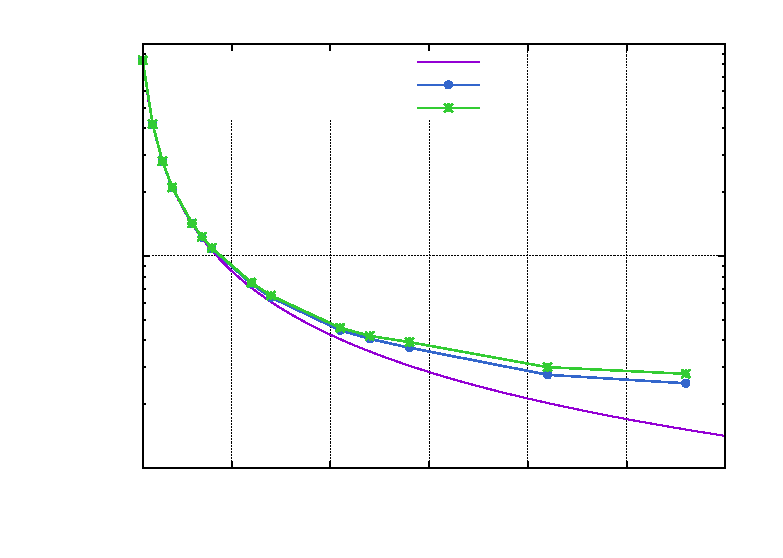
\includegraphics{plot-T-UDN-SM_nogatherInt_selected_500_selected_168}}%
    \gplfronttext
  \end{picture}%
\endgroup
}
      \caption{Dimensione della matrice 168x168}
      \label{fig:compare_s_sm_168}
    \end{subfigure}
    ~
    \begin{subfigure}[b]{\textwidth}
      \centering
      \addtocounter{subfigure}{-1}
      \renewcommand\thesubfigure{\alph{subfigure}3}
      \resizebox{\columnwidth}{!}{% GNUPLOT: LaTeX picture with Postscript
\begingroup
  \makeatletter
  \providecommand\color[2][]{%
    \GenericError{(gnuplot) \space\space\space\@spaces}{%
      Package color not loaded in conjunction with
      terminal option `colourtext'%
    }{See the gnuplot documentation for explanation.%
    }{Either use 'blacktext' in gnuplot or load the package
      color.sty in LaTeX.}%
    \renewcommand\color[2][]{}%
  }%
  \providecommand\includegraphics[2][]{%
    \GenericError{(gnuplot) \space\space\space\@spaces}{%
      Package graphicx or graphics not loaded%
    }{See the gnuplot documentation for explanation.%
    }{The gnuplot epslatex terminal needs graphicx.sty or graphics.sty.}%
    \renewcommand\includegraphics[2][]{}%
  }%
  \providecommand\rotatebox[2]{#2}%
  \@ifundefined{ifGPcolor}{%
    \newif\ifGPcolor
    \GPcolortrue
  }{}%
  \@ifundefined{ifGPblacktext}{%
    \newif\ifGPblacktext
    \GPblacktexttrue
  }{}%
  % define a \g@addto@macro without @ in the name:
  \let\gplgaddtomacro\g@addto@macro
  % define empty templates for all commands taking text:
  \gdef\gplbacktext{}%
  \gdef\gplfronttext{}%
  \makeatother
  \ifGPblacktext
    % no textcolor at all
    \def\colorrgb#1{}%
    \def\colorgray#1{}%
  \else
    % gray or color?
    \ifGPcolor
      \def\colorrgb#1{\color[rgb]{#1}}%
      \def\colorgray#1{\color[gray]{#1}}%
      \expandafter\def\csname LTw\endcsname{\color{white}}%
      \expandafter\def\csname LTb\endcsname{\color{black}}%
      \expandafter\def\csname LTa\endcsname{\color{black}}%
      \expandafter\def\csname LT0\endcsname{\color[rgb]{1,0,0}}%
      \expandafter\def\csname LT1\endcsname{\color[rgb]{0,1,0}}%
      \expandafter\def\csname LT2\endcsname{\color[rgb]{0,0,1}}%
      \expandafter\def\csname LT3\endcsname{\color[rgb]{1,0,1}}%
      \expandafter\def\csname LT4\endcsname{\color[rgb]{0,1,1}}%
      \expandafter\def\csname LT5\endcsname{\color[rgb]{1,1,0}}%
      \expandafter\def\csname LT6\endcsname{\color[rgb]{0,0,0}}%
      \expandafter\def\csname LT7\endcsname{\color[rgb]{1,0.3,0}}%
      \expandafter\def\csname LT8\endcsname{\color[rgb]{0.5,0.5,0.5}}%
    \else
      % gray
      \def\colorrgb#1{\color{black}}%
      \def\colorgray#1{\color[gray]{#1}}%
      \expandafter\def\csname LTw\endcsname{\color{white}}%
      \expandafter\def\csname LTb\endcsname{\color{black}}%
      \expandafter\def\csname LTa\endcsname{\color{black}}%
      \expandafter\def\csname LT0\endcsname{\color{black}}%
      \expandafter\def\csname LT1\endcsname{\color{black}}%
      \expandafter\def\csname LT2\endcsname{\color{black}}%
      \expandafter\def\csname LT3\endcsname{\color{black}}%
      \expandafter\def\csname LT4\endcsname{\color{black}}%
      \expandafter\def\csname LT5\endcsname{\color{black}}%
      \expandafter\def\csname LT6\endcsname{\color{black}}%
      \expandafter\def\csname LT7\endcsname{\color{black}}%
      \expandafter\def\csname LT8\endcsname{\color{black}}%
    \fi
  \fi
  \setlength{\unitlength}{0.0500bp}%
  \begin{picture}(7200.00,5040.00)%
    \gplgaddtomacro\gplbacktext{%
      \csname LTb\endcsname%
      \put(1210,704){\makebox(0,0)[r]{\strut{} 10}}%
      \csname LTb\endcsname%
      \put(1210,2061){\makebox(0,0)[r]{\strut{} 100}}%
      \csname LTb\endcsname%
      \put(1210,3418){\makebox(0,0)[r]{\strut{} 1000}}%
      \csname LTb\endcsname%
      \put(1210,4775){\makebox(0,0)[r]{\strut{} 10000}}%
      \csname LTb\endcsname%
      \put(2175,484){\makebox(0,0){\strut{} 10}}%
      \csname LTb\endcsname%
      \put(3101,484){\makebox(0,0){\strut{} 20}}%
      \csname LTb\endcsname%
      \put(4026,484){\makebox(0,0){\strut{} 30}}%
      \csname LTb\endcsname%
      \put(4952,484){\makebox(0,0){\strut{} 40}}%
      \csname LTb\endcsname%
      \put(5877,484){\makebox(0,0){\strut{} 50}}%
      \csname LTb\endcsname%
      \put(6803,484){\makebox(0,0){\strut{} 60}}%
      \put(176,2739){\rotatebox{-270}{\makebox(0,0){\strut{}service time ($\,\mu\mathrm{sec}$\,)}}}%
      \put(4072,154){\makebox(0,0){\strut{}$n$ parallel degree}}%
    }%
    \gplgaddtomacro\gplfronttext{%
      \csname LTb\endcsname%
      \put(3850,4602){\makebox(0,0)[r]{\strut{}ideal service time}}%
      \csname LTb\endcsname%
      \put(3850,4382){\makebox(0,0)[r]{\strut{}udn udn}}%
      \csname LTb\endcsname%
      \put(3850,4162){\makebox(0,0)[r]{\strut{}sm sm}}%
    }%
    \gplbacktext
    \put(0,0){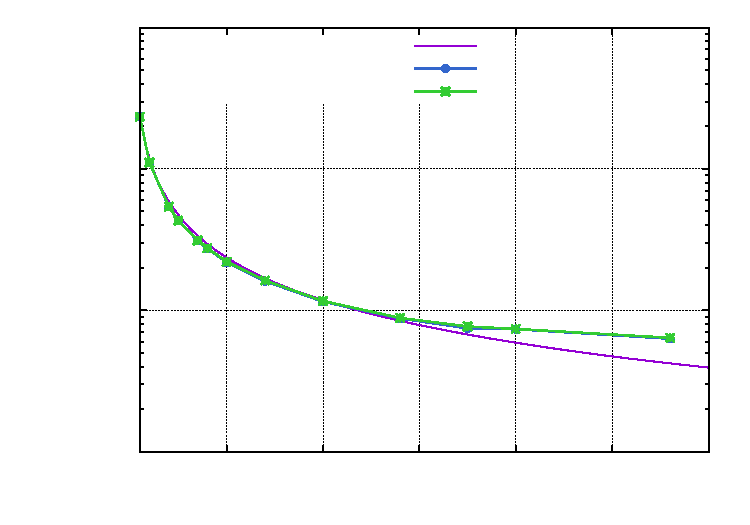
\includegraphics{plot-T-UDN-SM_nogatherInt_selected_500_selected_280}}%
    \gplfronttext
  \end{picture}%
\endgroup
}
      \caption{Dimensione della matrice 280x280}
      \label{fig:compare_s_sm_280}
    \end{subfigure}
    \label{fig:compare_s_sm}
  \end{subfigure}
  \label{fig:compare}
\end{figure}




%% \begin{figure}[p]
%%   \centering
%%   \begin{subfigure}[b]{.31\textheight}
%%     \centering
%%     \resizebox{\columnwidth}{!}{% GNUPLOT: LaTeX picture with Postscript
\begingroup
  \makeatletter
  \providecommand\color[2][]{%
    \GenericError{(gnuplot) \space\space\space\@spaces}{%
      Package color not loaded in conjunction with
      terminal option `colourtext'%
    }{See the gnuplot documentation for explanation.%
    }{Either use 'blacktext' in gnuplot or load the package
      color.sty in LaTeX.}%
    \renewcommand\color[2][]{}%
  }%
  \providecommand\includegraphics[2][]{%
    \GenericError{(gnuplot) \space\space\space\@spaces}{%
      Package graphicx or graphics not loaded%
    }{See the gnuplot documentation for explanation.%
    }{The gnuplot epslatex terminal needs graphicx.sty or graphics.sty.}%
    \renewcommand\includegraphics[2][]{}%
  }%
  \providecommand\rotatebox[2]{#2}%
  \@ifundefined{ifGPcolor}{%
    \newif\ifGPcolor
    \GPcolortrue
  }{}%
  \@ifundefined{ifGPblacktext}{%
    \newif\ifGPblacktext
    \GPblacktexttrue
  }{}%
  % define a \g@addto@macro without @ in the name:
  \let\gplgaddtomacro\g@addto@macro
  % define empty templates for all commands taking text:
  \gdef\gplbacktext{}%
  \gdef\gplfronttext{}%
  \makeatother
  \ifGPblacktext
    % no textcolor at all
    \def\colorrgb#1{}%
    \def\colorgray#1{}%
  \else
    % gray or color?
    \ifGPcolor
      \def\colorrgb#1{\color[rgb]{#1}}%
      \def\colorgray#1{\color[gray]{#1}}%
      \expandafter\def\csname LTw\endcsname{\color{white}}%
      \expandafter\def\csname LTb\endcsname{\color{black}}%
      \expandafter\def\csname LTa\endcsname{\color{black}}%
      \expandafter\def\csname LT0\endcsname{\color[rgb]{1,0,0}}%
      \expandafter\def\csname LT1\endcsname{\color[rgb]{0,1,0}}%
      \expandafter\def\csname LT2\endcsname{\color[rgb]{0,0,1}}%
      \expandafter\def\csname LT3\endcsname{\color[rgb]{1,0,1}}%
      \expandafter\def\csname LT4\endcsname{\color[rgb]{0,1,1}}%
      \expandafter\def\csname LT5\endcsname{\color[rgb]{1,1,0}}%
      \expandafter\def\csname LT6\endcsname{\color[rgb]{0,0,0}}%
      \expandafter\def\csname LT7\endcsname{\color[rgb]{1,0.3,0}}%
      \expandafter\def\csname LT8\endcsname{\color[rgb]{0.5,0.5,0.5}}%
    \else
      % gray
      \def\colorrgb#1{\color{black}}%
      \def\colorgray#1{\color[gray]{#1}}%
      \expandafter\def\csname LTw\endcsname{\color{white}}%
      \expandafter\def\csname LTb\endcsname{\color{black}}%
      \expandafter\def\csname LTa\endcsname{\color{black}}%
      \expandafter\def\csname LT0\endcsname{\color{black}}%
      \expandafter\def\csname LT1\endcsname{\color{black}}%
      \expandafter\def\csname LT2\endcsname{\color{black}}%
      \expandafter\def\csname LT3\endcsname{\color{black}}%
      \expandafter\def\csname LT4\endcsname{\color{black}}%
      \expandafter\def\csname LT5\endcsname{\color{black}}%
      \expandafter\def\csname LT6\endcsname{\color{black}}%
      \expandafter\def\csname LT7\endcsname{\color{black}}%
      \expandafter\def\csname LT8\endcsname{\color{black}}%
    \fi
  \fi
  \setlength{\unitlength}{0.0500bp}%
  \begin{picture}(7200.00,5040.00)%
    \gplgaddtomacro\gplbacktext{%
      \csname LTb\endcsname%
      \put(814,1325){\makebox(0,0)[r]{\strut{} 10}}%
      \put(814,2015){\makebox(0,0)[r]{\strut{} 20}}%
      \put(814,2705){\makebox(0,0)[r]{\strut{} 30}}%
      \put(814,3395){\makebox(0,0)[r]{\strut{} 40}}%
      \put(814,4085){\makebox(0,0)[r]{\strut{} 50}}%
      \put(814,4775){\makebox(0,0)[r]{\strut{} 60}}%
      \put(1839,484){\makebox(0,0){\strut{} 10}}%
      \put(2832,484){\makebox(0,0){\strut{} 20}}%
      \put(3825,484){\makebox(0,0){\strut{} 30}}%
      \put(4818,484){\makebox(0,0){\strut{} 40}}%
      \put(5810,484){\makebox(0,0){\strut{} 50}}%
      \put(6803,484){\makebox(0,0){\strut{} 60}}%
      \put(176,2739){\rotatebox{-270}{\makebox(0,0){\strut{}scalability}}}%
      \put(3874,154){\makebox(0,0){\strut{}$n$ parallel degree}}%
    }%
    \gplgaddtomacro\gplfronttext{%
      \csname LTb\endcsname%
      \put(3322,4602){\makebox(0,0)[r]{\strut{}ideal scalability}}%
      \csname LTb\endcsname%
      \put(3322,4382){\makebox(0,0)[r]{\strut{}udn udn}}%
      \csname LTb\endcsname%
      \put(3322,4162){\makebox(0,0)[r]{\strut{}sm sm}}%
    }%
    \gplbacktext
    \put(0,0){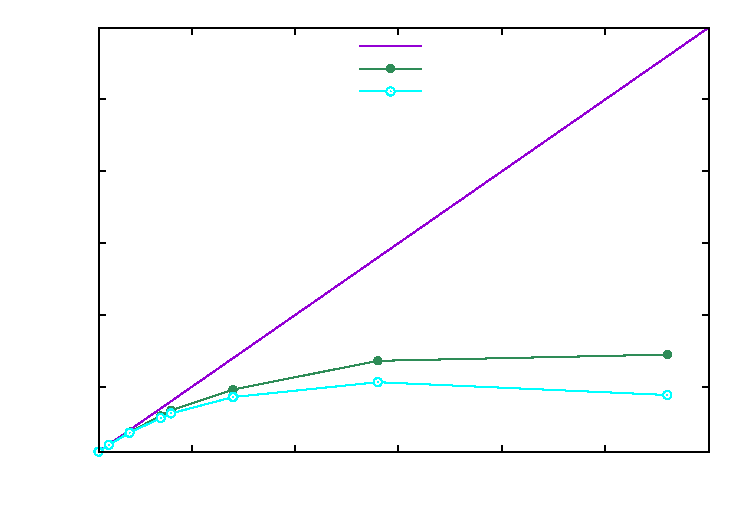
\includegraphics{plot-comp-Tc-s_nogatherInt_all_500_181_56}}%
    \gplfronttext
  \end{picture}%
\endgroup
}
%%     \caption{Confronto della scalabilita nelle diverse implementazioni, Ta=181, M=56}
%%   \end{subfigure}
%%   \vfill
%%   %%\vspace{5ex}
%%   \begin{subfigure}[b]{.31\textheight}
%%     \centering
%%     \resizebox{\columnwidth}{!}{% GNUPLOT: LaTeX picture with Postscript
\begingroup
  \makeatletter
  \providecommand\color[2][]{%
    \GenericError{(gnuplot) \space\space\space\@spaces}{%
      Package color not loaded in conjunction with
      terminal option `colourtext'%
    }{See the gnuplot documentation for explanation.%
    }{Either use 'blacktext' in gnuplot or load the package
      color.sty in LaTeX.}%
    \renewcommand\color[2][]{}%
  }%
  \providecommand\includegraphics[2][]{%
    \GenericError{(gnuplot) \space\space\space\@spaces}{%
      Package graphicx or graphics not loaded%
    }{See the gnuplot documentation for explanation.%
    }{The gnuplot epslatex terminal needs graphicx.sty or graphics.sty.}%
    \renewcommand\includegraphics[2][]{}%
  }%
  \providecommand\rotatebox[2]{#2}%
  \@ifundefined{ifGPcolor}{%
    \newif\ifGPcolor
    \GPcolortrue
  }{}%
  \@ifundefined{ifGPblacktext}{%
    \newif\ifGPblacktext
    \GPblacktexttrue
  }{}%
  % define a \g@addto@macro without @ in the name:
  \let\gplgaddtomacro\g@addto@macro
  % define empty templates for all commands taking text:
  \gdef\gplbacktext{}%
  \gdef\gplfronttext{}%
  \makeatother
  \ifGPblacktext
    % no textcolor at all
    \def\colorrgb#1{}%
    \def\colorgray#1{}%
  \else
    % gray or color?
    \ifGPcolor
      \def\colorrgb#1{\color[rgb]{#1}}%
      \def\colorgray#1{\color[gray]{#1}}%
      \expandafter\def\csname LTw\endcsname{\color{white}}%
      \expandafter\def\csname LTb\endcsname{\color{black}}%
      \expandafter\def\csname LTa\endcsname{\color{black}}%
      \expandafter\def\csname LT0\endcsname{\color[rgb]{1,0,0}}%
      \expandafter\def\csname LT1\endcsname{\color[rgb]{0,1,0}}%
      \expandafter\def\csname LT2\endcsname{\color[rgb]{0,0,1}}%
      \expandafter\def\csname LT3\endcsname{\color[rgb]{1,0,1}}%
      \expandafter\def\csname LT4\endcsname{\color[rgb]{0,1,1}}%
      \expandafter\def\csname LT5\endcsname{\color[rgb]{1,1,0}}%
      \expandafter\def\csname LT6\endcsname{\color[rgb]{0,0,0}}%
      \expandafter\def\csname LT7\endcsname{\color[rgb]{1,0.3,0}}%
      \expandafter\def\csname LT8\endcsname{\color[rgb]{0.5,0.5,0.5}}%
    \else
      % gray
      \def\colorrgb#1{\color{black}}%
      \def\colorgray#1{\color[gray]{#1}}%
      \expandafter\def\csname LTw\endcsname{\color{white}}%
      \expandafter\def\csname LTb\endcsname{\color{black}}%
      \expandafter\def\csname LTa\endcsname{\color{black}}%
      \expandafter\def\csname LT0\endcsname{\color{black}}%
      \expandafter\def\csname LT1\endcsname{\color{black}}%
      \expandafter\def\csname LT2\endcsname{\color{black}}%
      \expandafter\def\csname LT3\endcsname{\color{black}}%
      \expandafter\def\csname LT4\endcsname{\color{black}}%
      \expandafter\def\csname LT5\endcsname{\color{black}}%
      \expandafter\def\csname LT6\endcsname{\color{black}}%
      \expandafter\def\csname LT7\endcsname{\color{black}}%
      \expandafter\def\csname LT8\endcsname{\color{black}}%
    \fi
  \fi
  \setlength{\unitlength}{0.0500bp}%
  \begin{picture}(7200.00,5040.00)%
    \gplgaddtomacro\gplbacktext{%
      \csname LTb\endcsname%
      \put(814,1325){\makebox(0,0)[r]{\strut{} 10}}%
      \put(814,2015){\makebox(0,0)[r]{\strut{} 20}}%
      \put(814,2705){\makebox(0,0)[r]{\strut{} 30}}%
      \put(814,3395){\makebox(0,0)[r]{\strut{} 40}}%
      \put(814,4085){\makebox(0,0)[r]{\strut{} 50}}%
      \put(814,4775){\makebox(0,0)[r]{\strut{} 60}}%
      \put(1839,484){\makebox(0,0){\strut{} 10}}%
      \put(2832,484){\makebox(0,0){\strut{} 20}}%
      \put(3825,484){\makebox(0,0){\strut{} 30}}%
      \put(4818,484){\makebox(0,0){\strut{} 40}}%
      \put(5810,484){\makebox(0,0){\strut{} 50}}%
      \put(6803,484){\makebox(0,0){\strut{} 60}}%
      \put(176,2739){\rotatebox{-270}{\makebox(0,0){\strut{}scalability}}}%
      \put(3874,154){\makebox(0,0){\strut{}$n$ parallel degree}}%
    }%
    \gplgaddtomacro\gplfronttext{%
      \csname LTb\endcsname%
      \put(3322,4602){\makebox(0,0)[r]{\strut{}ideal scalability}}%
      \csname LTb\endcsname%
      \put(3322,4382){\makebox(0,0)[r]{\strut{}udn udn}}%
      \csname LTb\endcsname%
      \put(3322,4162){\makebox(0,0)[r]{\strut{}sm sm}}%
    }%
    \gplbacktext
    \put(0,0){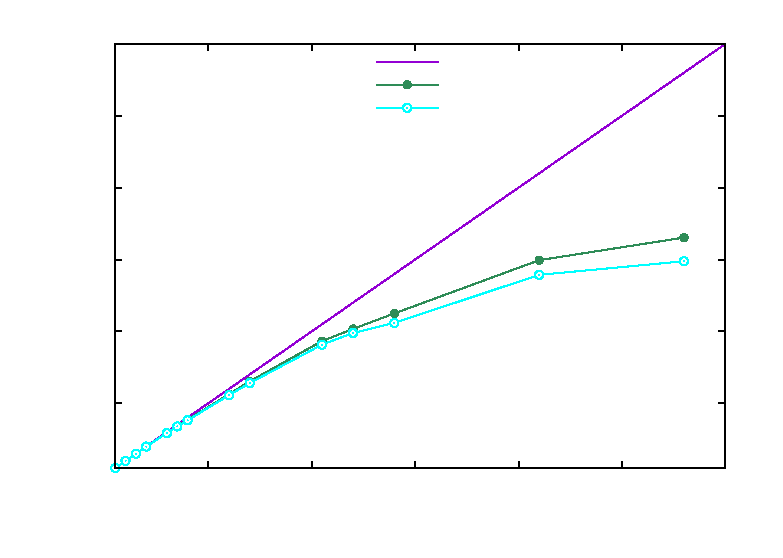
\includegraphics{plot-comp-Tc-s_nogatherInt_all_500_181_168}}%
    \gplfronttext
  \end{picture}%
\endgroup
}
%%     \caption{Confronto della scalabilita nelle diverse implementazioni, Ta=181, M=168}
%%   \end{subfigure}
%%   \vfill
%%   \begin{subfigure}[b]{.31\textheight}
%%     \centering
%%     \resizebox{\columnwidth}{!}{% GNUPLOT: LaTeX picture with Postscript
\begingroup
  \makeatletter
  \providecommand\color[2][]{%
    \GenericError{(gnuplot) \space\space\space\@spaces}{%
      Package color not loaded in conjunction with
      terminal option `colourtext'%
    }{See the gnuplot documentation for explanation.%
    }{Either use 'blacktext' in gnuplot or load the package
      color.sty in LaTeX.}%
    \renewcommand\color[2][]{}%
  }%
  \providecommand\includegraphics[2][]{%
    \GenericError{(gnuplot) \space\space\space\@spaces}{%
      Package graphicx or graphics not loaded%
    }{See the gnuplot documentation for explanation.%
    }{The gnuplot epslatex terminal needs graphicx.sty or graphics.sty.}%
    \renewcommand\includegraphics[2][]{}%
  }%
  \providecommand\rotatebox[2]{#2}%
  \@ifundefined{ifGPcolor}{%
    \newif\ifGPcolor
    \GPcolortrue
  }{}%
  \@ifundefined{ifGPblacktext}{%
    \newif\ifGPblacktext
    \GPblacktexttrue
  }{}%
  % define a \g@addto@macro without @ in the name:
  \let\gplgaddtomacro\g@addto@macro
  % define empty templates for all commands taking text:
  \gdef\gplbacktext{}%
  \gdef\gplfronttext{}%
  \makeatother
  \ifGPblacktext
    % no textcolor at all
    \def\colorrgb#1{}%
    \def\colorgray#1{}%
  \else
    % gray or color?
    \ifGPcolor
      \def\colorrgb#1{\color[rgb]{#1}}%
      \def\colorgray#1{\color[gray]{#1}}%
      \expandafter\def\csname LTw\endcsname{\color{white}}%
      \expandafter\def\csname LTb\endcsname{\color{black}}%
      \expandafter\def\csname LTa\endcsname{\color{black}}%
      \expandafter\def\csname LT0\endcsname{\color[rgb]{1,0,0}}%
      \expandafter\def\csname LT1\endcsname{\color[rgb]{0,1,0}}%
      \expandafter\def\csname LT2\endcsname{\color[rgb]{0,0,1}}%
      \expandafter\def\csname LT3\endcsname{\color[rgb]{1,0,1}}%
      \expandafter\def\csname LT4\endcsname{\color[rgb]{0,1,1}}%
      \expandafter\def\csname LT5\endcsname{\color[rgb]{1,1,0}}%
      \expandafter\def\csname LT6\endcsname{\color[rgb]{0,0,0}}%
      \expandafter\def\csname LT7\endcsname{\color[rgb]{1,0.3,0}}%
      \expandafter\def\csname LT8\endcsname{\color[rgb]{0.5,0.5,0.5}}%
    \else
      % gray
      \def\colorrgb#1{\color{black}}%
      \def\colorgray#1{\color[gray]{#1}}%
      \expandafter\def\csname LTw\endcsname{\color{white}}%
      \expandafter\def\csname LTb\endcsname{\color{black}}%
      \expandafter\def\csname LTa\endcsname{\color{black}}%
      \expandafter\def\csname LT0\endcsname{\color{black}}%
      \expandafter\def\csname LT1\endcsname{\color{black}}%
      \expandafter\def\csname LT2\endcsname{\color{black}}%
      \expandafter\def\csname LT3\endcsname{\color{black}}%
      \expandafter\def\csname LT4\endcsname{\color{black}}%
      \expandafter\def\csname LT5\endcsname{\color{black}}%
      \expandafter\def\csname LT6\endcsname{\color{black}}%
      \expandafter\def\csname LT7\endcsname{\color{black}}%
      \expandafter\def\csname LT8\endcsname{\color{black}}%
    \fi
  \fi
  \setlength{\unitlength}{0.0500bp}%
  \begin{picture}(7200.00,5040.00)%
    \gplgaddtomacro\gplbacktext{%
      \csname LTb\endcsname%
      \put(814,1325){\makebox(0,0)[r]{\strut{} 10}}%
      \put(814,2015){\makebox(0,0)[r]{\strut{} 20}}%
      \put(814,2705){\makebox(0,0)[r]{\strut{} 30}}%
      \put(814,3395){\makebox(0,0)[r]{\strut{} 40}}%
      \put(814,4085){\makebox(0,0)[r]{\strut{} 50}}%
      \put(814,4775){\makebox(0,0)[r]{\strut{} 60}}%
      \put(1839,484){\makebox(0,0){\strut{} 10}}%
      \put(2832,484){\makebox(0,0){\strut{} 20}}%
      \put(3825,484){\makebox(0,0){\strut{} 30}}%
      \put(4818,484){\makebox(0,0){\strut{} 40}}%
      \put(5810,484){\makebox(0,0){\strut{} 50}}%
      \put(6803,484){\makebox(0,0){\strut{} 60}}%
      \put(176,2739){\rotatebox{-270}{\makebox(0,0){\strut{}scalability}}}%
      \put(3874,154){\makebox(0,0){\strut{}$n$ parallel degree}}%
    }%
    \gplgaddtomacro\gplfronttext{%
      \csname LTb\endcsname%
      \put(3322,4602){\makebox(0,0)[r]{\strut{}ideal scalability}}%
      \csname LTb\endcsname%
      \put(3322,4382){\makebox(0,0)[r]{\strut{}udn udn}}%
      \csname LTb\endcsname%
      \put(3322,4162){\makebox(0,0)[r]{\strut{}sm sm}}%
    }%
    \gplbacktext
    \put(0,0){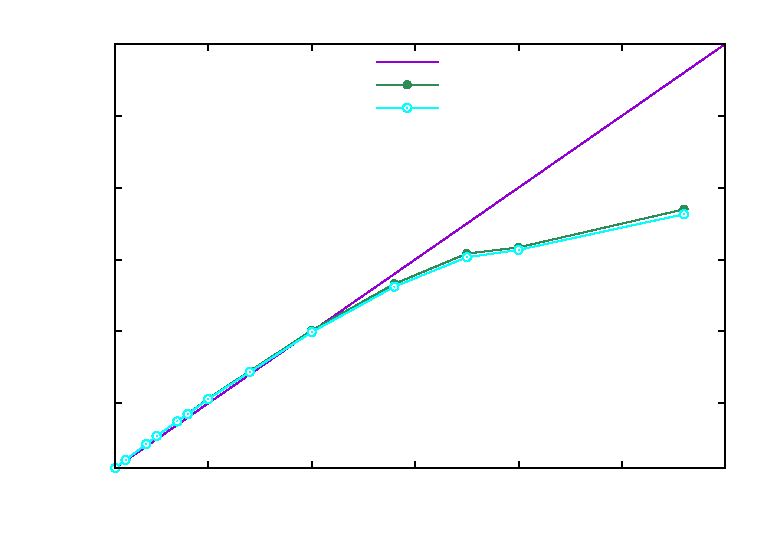
\includegraphics{plot-comp-Tc-s_nogatherInt_all_500_181_280}}%
    \gplfronttext
  \end{picture}%
\endgroup
}
%%     \caption{Confronto della scalabilita nelle diverse implementazioni, Ta=181, M=280}
%%   \end{subfigure}
%% \end{figure}

%% \begin{figure}[p]
%%   \centering
%%   \begin{subfigure}[b]{.31\textheight}
%%     \centering
%%     \resizebox{\columnwidth}{!}{% GNUPLOT: LaTeX picture with Postscript
\begingroup
  \makeatletter
  \providecommand\color[2][]{%
    \GenericError{(gnuplot) \space\space\space\@spaces}{%
      Package color not loaded in conjunction with
      terminal option `colourtext'%
    }{See the gnuplot documentation for explanation.%
    }{Either use 'blacktext' in gnuplot or load the package
      color.sty in LaTeX.}%
    \renewcommand\color[2][]{}%
  }%
  \providecommand\includegraphics[2][]{%
    \GenericError{(gnuplot) \space\space\space\@spaces}{%
      Package graphicx or graphics not loaded%
    }{See the gnuplot documentation for explanation.%
    }{The gnuplot epslatex terminal needs graphicx.sty or graphics.sty.}%
    \renewcommand\includegraphics[2][]{}%
  }%
  \providecommand\rotatebox[2]{#2}%
  \@ifundefined{ifGPcolor}{%
    \newif\ifGPcolor
    \GPcolortrue
  }{}%
  \@ifundefined{ifGPblacktext}{%
    \newif\ifGPblacktext
    \GPblacktexttrue
  }{}%
  % define a \g@addto@macro without @ in the name:
  \let\gplgaddtomacro\g@addto@macro
  % define empty templates for all commands taking text:
  \gdef\gplbacktext{}%
  \gdef\gplfronttext{}%
  \makeatother
  \ifGPblacktext
    % no textcolor at all
    \def\colorrgb#1{}%
    \def\colorgray#1{}%
  \else
    % gray or color?
    \ifGPcolor
      \def\colorrgb#1{\color[rgb]{#1}}%
      \def\colorgray#1{\color[gray]{#1}}%
      \expandafter\def\csname LTw\endcsname{\color{white}}%
      \expandafter\def\csname LTb\endcsname{\color{black}}%
      \expandafter\def\csname LTa\endcsname{\color{black}}%
      \expandafter\def\csname LT0\endcsname{\color[rgb]{1,0,0}}%
      \expandafter\def\csname LT1\endcsname{\color[rgb]{0,1,0}}%
      \expandafter\def\csname LT2\endcsname{\color[rgb]{0,0,1}}%
      \expandafter\def\csname LT3\endcsname{\color[rgb]{1,0,1}}%
      \expandafter\def\csname LT4\endcsname{\color[rgb]{0,1,1}}%
      \expandafter\def\csname LT5\endcsname{\color[rgb]{1,1,0}}%
      \expandafter\def\csname LT6\endcsname{\color[rgb]{0,0,0}}%
      \expandafter\def\csname LT7\endcsname{\color[rgb]{1,0.3,0}}%
      \expandafter\def\csname LT8\endcsname{\color[rgb]{0.5,0.5,0.5}}%
    \else
      % gray
      \def\colorrgb#1{\color{black}}%
      \def\colorgray#1{\color[gray]{#1}}%
      \expandafter\def\csname LTw\endcsname{\color{white}}%
      \expandafter\def\csname LTb\endcsname{\color{black}}%
      \expandafter\def\csname LTa\endcsname{\color{black}}%
      \expandafter\def\csname LT0\endcsname{\color{black}}%
      \expandafter\def\csname LT1\endcsname{\color{black}}%
      \expandafter\def\csname LT2\endcsname{\color{black}}%
      \expandafter\def\csname LT3\endcsname{\color{black}}%
      \expandafter\def\csname LT4\endcsname{\color{black}}%
      \expandafter\def\csname LT5\endcsname{\color{black}}%
      \expandafter\def\csname LT6\endcsname{\color{black}}%
      \expandafter\def\csname LT7\endcsname{\color{black}}%
      \expandafter\def\csname LT8\endcsname{\color{black}}%
    \fi
  \fi
  \setlength{\unitlength}{0.0500bp}%
  \begin{picture}(7200.00,5040.00)%
    \gplgaddtomacro\gplbacktext{%
      \csname LTb\endcsname%
      \put(946,704){\makebox(0,0)[r]{\strut{} 1}}%
      \csname LTb\endcsname%
      \put(946,2740){\makebox(0,0)[r]{\strut{} 10}}%
      \csname LTb\endcsname%
      \put(946,4775){\makebox(0,0)[r]{\strut{} 100}}%
      \csname LTb\endcsname%
      \put(1951,484){\makebox(0,0){\strut{} 10}}%
      \csname LTb\endcsname%
      \put(2922,484){\makebox(0,0){\strut{} 20}}%
      \csname LTb\endcsname%
      \put(3892,484){\makebox(0,0){\strut{} 30}}%
      \csname LTb\endcsname%
      \put(4862,484){\makebox(0,0){\strut{} 40}}%
      \csname LTb\endcsname%
      \put(5833,484){\makebox(0,0){\strut{} 50}}%
      \csname LTb\endcsname%
      \put(6803,484){\makebox(0,0){\strut{} 60}}%
      \put(176,2739){\rotatebox{-270}{\makebox(0,0){\strut{}service time ($\,\mu\mathrm{sec}$\,)}}}%
      \put(3940,154){\makebox(0,0){\strut{}$n$ parallel degree}}%
    }%
    \gplgaddtomacro\gplfronttext{%
      \csname LTb\endcsname%
      \put(3586,4602){\makebox(0,0)[r]{\strut{}ideal service time}}%
      \csname LTb\endcsname%
      \put(3586,4382){\makebox(0,0)[r]{\strut{}udn udn}}%
      \csname LTb\endcsname%
      \put(3586,4162){\makebox(0,0)[r]{\strut{}sm sm}}%
    }%
    \gplbacktext
    \put(0,0){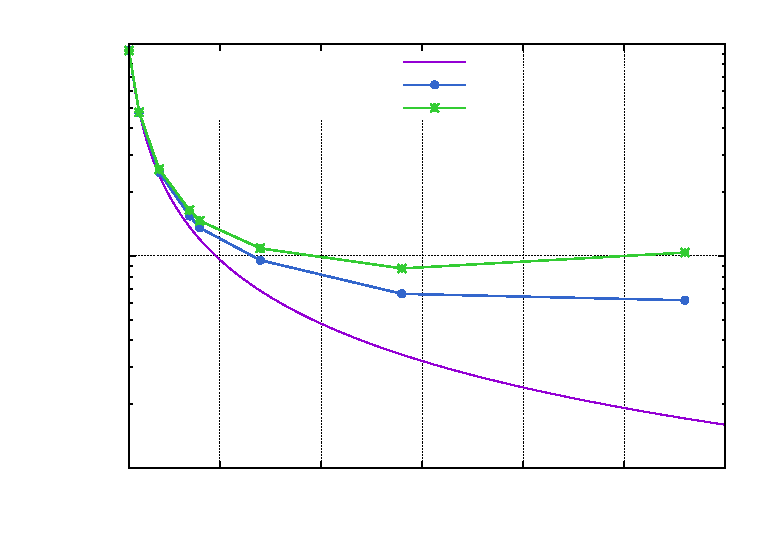
\includegraphics{plot-T-UDN-SM_nogatherInt_selected_500_selected_56}}%
    \gplfronttext
  \end{picture}%
\endgroup
}
%%     \caption{Confronto della scalabilita nelle diverse implementazioni, Ta=181, M=56}
%%   \end{subfigure}
%%   \vfill
%%   %%\vspace{5ex}
%%   \begin{subfigure}[b]{.31\textheight}
%%     \centering
%%     \resizebox{\columnwidth}{!}{% GNUPLOT: LaTeX picture with Postscript
\begingroup
  \makeatletter
  \providecommand\color[2][]{%
    \GenericError{(gnuplot) \space\space\space\@spaces}{%
      Package color not loaded in conjunction with
      terminal option `colourtext'%
    }{See the gnuplot documentation for explanation.%
    }{Either use 'blacktext' in gnuplot or load the package
      color.sty in LaTeX.}%
    \renewcommand\color[2][]{}%
  }%
  \providecommand\includegraphics[2][]{%
    \GenericError{(gnuplot) \space\space\space\@spaces}{%
      Package graphicx or graphics not loaded%
    }{See the gnuplot documentation for explanation.%
    }{The gnuplot epslatex terminal needs graphicx.sty or graphics.sty.}%
    \renewcommand\includegraphics[2][]{}%
  }%
  \providecommand\rotatebox[2]{#2}%
  \@ifundefined{ifGPcolor}{%
    \newif\ifGPcolor
    \GPcolortrue
  }{}%
  \@ifundefined{ifGPblacktext}{%
    \newif\ifGPblacktext
    \GPblacktexttrue
  }{}%
  % define a \g@addto@macro without @ in the name:
  \let\gplgaddtomacro\g@addto@macro
  % define empty templates for all commands taking text:
  \gdef\gplbacktext{}%
  \gdef\gplfronttext{}%
  \makeatother
  \ifGPblacktext
    % no textcolor at all
    \def\colorrgb#1{}%
    \def\colorgray#1{}%
  \else
    % gray or color?
    \ifGPcolor
      \def\colorrgb#1{\color[rgb]{#1}}%
      \def\colorgray#1{\color[gray]{#1}}%
      \expandafter\def\csname LTw\endcsname{\color{white}}%
      \expandafter\def\csname LTb\endcsname{\color{black}}%
      \expandafter\def\csname LTa\endcsname{\color{black}}%
      \expandafter\def\csname LT0\endcsname{\color[rgb]{1,0,0}}%
      \expandafter\def\csname LT1\endcsname{\color[rgb]{0,1,0}}%
      \expandafter\def\csname LT2\endcsname{\color[rgb]{0,0,1}}%
      \expandafter\def\csname LT3\endcsname{\color[rgb]{1,0,1}}%
      \expandafter\def\csname LT4\endcsname{\color[rgb]{0,1,1}}%
      \expandafter\def\csname LT5\endcsname{\color[rgb]{1,1,0}}%
      \expandafter\def\csname LT6\endcsname{\color[rgb]{0,0,0}}%
      \expandafter\def\csname LT7\endcsname{\color[rgb]{1,0.3,0}}%
      \expandafter\def\csname LT8\endcsname{\color[rgb]{0.5,0.5,0.5}}%
    \else
      % gray
      \def\colorrgb#1{\color{black}}%
      \def\colorgray#1{\color[gray]{#1}}%
      \expandafter\def\csname LTw\endcsname{\color{white}}%
      \expandafter\def\csname LTb\endcsname{\color{black}}%
      \expandafter\def\csname LTa\endcsname{\color{black}}%
      \expandafter\def\csname LT0\endcsname{\color{black}}%
      \expandafter\def\csname LT1\endcsname{\color{black}}%
      \expandafter\def\csname LT2\endcsname{\color{black}}%
      \expandafter\def\csname LT3\endcsname{\color{black}}%
      \expandafter\def\csname LT4\endcsname{\color{black}}%
      \expandafter\def\csname LT5\endcsname{\color{black}}%
      \expandafter\def\csname LT6\endcsname{\color{black}}%
      \expandafter\def\csname LT7\endcsname{\color{black}}%
      \expandafter\def\csname LT8\endcsname{\color{black}}%
    \fi
  \fi
  \setlength{\unitlength}{0.0500bp}%
  \begin{picture}(7200.00,5040.00)%
    \gplgaddtomacro\gplbacktext{%
      \csname LTb\endcsname%
      \put(1078,704){\makebox(0,0)[r]{\strut{} 10}}%
      \csname LTb\endcsname%
      \put(1078,2740){\makebox(0,0)[r]{\strut{} 100}}%
      \csname LTb\endcsname%
      \put(1078,4775){\makebox(0,0)[r]{\strut{} 1000}}%
      \csname LTb\endcsname%
      \put(2063,484){\makebox(0,0){\strut{} 10}}%
      \csname LTb\endcsname%
      \put(3011,484){\makebox(0,0){\strut{} 20}}%
      \csname LTb\endcsname%
      \put(3959,484){\makebox(0,0){\strut{} 30}}%
      \csname LTb\endcsname%
      \put(4907,484){\makebox(0,0){\strut{} 40}}%
      \csname LTb\endcsname%
      \put(5855,484){\makebox(0,0){\strut{} 50}}%
      \csname LTb\endcsname%
      \put(6803,484){\makebox(0,0){\strut{} 60}}%
      \put(176,2739){\rotatebox{-270}{\makebox(0,0){\strut{}service time ($\,\mu\mathrm{sec}$\,)}}}%
      \put(4006,154){\makebox(0,0){\strut{}$n$ parallel degree}}%
    }%
    \gplgaddtomacro\gplfronttext{%
      \csname LTb\endcsname%
      \put(3718,4602){\makebox(0,0)[r]{\strut{}ideal service time}}%
      \csname LTb\endcsname%
      \put(3718,4382){\makebox(0,0)[r]{\strut{}udn udn}}%
      \csname LTb\endcsname%
      \put(3718,4162){\makebox(0,0)[r]{\strut{}sm sm}}%
    }%
    \gplbacktext
    \put(0,0){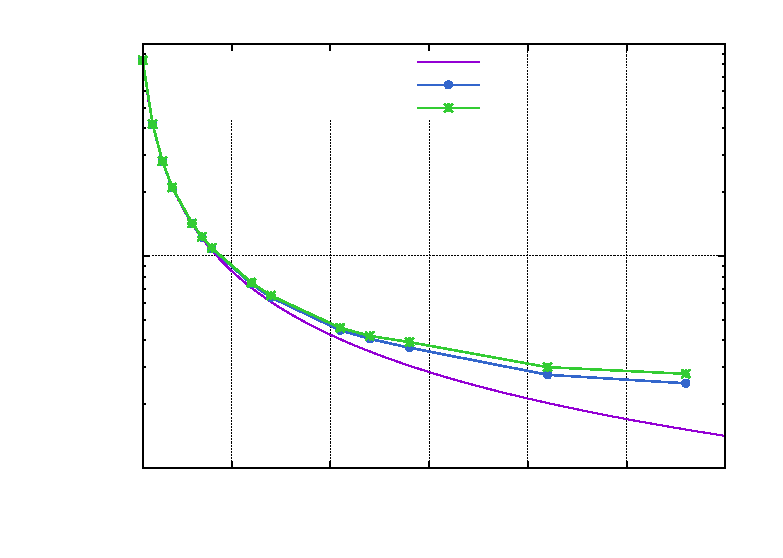
\includegraphics{plot-T-UDN-SM_nogatherInt_selected_500_selected_168}}%
    \gplfronttext
  \end{picture}%
\endgroup
}
%%     \caption{Confronto della scalabilita nelle diverse implementazioni, Ta=181, M=168}
%%   \end{subfigure}
%%   \vfill
%%   \begin{subfigure}[b]{.31\textheight}
%%     \centering
%%     \resizebox{\columnwidth}{!}{% GNUPLOT: LaTeX picture with Postscript
\begingroup
  \makeatletter
  \providecommand\color[2][]{%
    \GenericError{(gnuplot) \space\space\space\@spaces}{%
      Package color not loaded in conjunction with
      terminal option `colourtext'%
    }{See the gnuplot documentation for explanation.%
    }{Either use 'blacktext' in gnuplot or load the package
      color.sty in LaTeX.}%
    \renewcommand\color[2][]{}%
  }%
  \providecommand\includegraphics[2][]{%
    \GenericError{(gnuplot) \space\space\space\@spaces}{%
      Package graphicx or graphics not loaded%
    }{See the gnuplot documentation for explanation.%
    }{The gnuplot epslatex terminal needs graphicx.sty or graphics.sty.}%
    \renewcommand\includegraphics[2][]{}%
  }%
  \providecommand\rotatebox[2]{#2}%
  \@ifundefined{ifGPcolor}{%
    \newif\ifGPcolor
    \GPcolortrue
  }{}%
  \@ifundefined{ifGPblacktext}{%
    \newif\ifGPblacktext
    \GPblacktexttrue
  }{}%
  % define a \g@addto@macro without @ in the name:
  \let\gplgaddtomacro\g@addto@macro
  % define empty templates for all commands taking text:
  \gdef\gplbacktext{}%
  \gdef\gplfronttext{}%
  \makeatother
  \ifGPblacktext
    % no textcolor at all
    \def\colorrgb#1{}%
    \def\colorgray#1{}%
  \else
    % gray or color?
    \ifGPcolor
      \def\colorrgb#1{\color[rgb]{#1}}%
      \def\colorgray#1{\color[gray]{#1}}%
      \expandafter\def\csname LTw\endcsname{\color{white}}%
      \expandafter\def\csname LTb\endcsname{\color{black}}%
      \expandafter\def\csname LTa\endcsname{\color{black}}%
      \expandafter\def\csname LT0\endcsname{\color[rgb]{1,0,0}}%
      \expandafter\def\csname LT1\endcsname{\color[rgb]{0,1,0}}%
      \expandafter\def\csname LT2\endcsname{\color[rgb]{0,0,1}}%
      \expandafter\def\csname LT3\endcsname{\color[rgb]{1,0,1}}%
      \expandafter\def\csname LT4\endcsname{\color[rgb]{0,1,1}}%
      \expandafter\def\csname LT5\endcsname{\color[rgb]{1,1,0}}%
      \expandafter\def\csname LT6\endcsname{\color[rgb]{0,0,0}}%
      \expandafter\def\csname LT7\endcsname{\color[rgb]{1,0.3,0}}%
      \expandafter\def\csname LT8\endcsname{\color[rgb]{0.5,0.5,0.5}}%
    \else
      % gray
      \def\colorrgb#1{\color{black}}%
      \def\colorgray#1{\color[gray]{#1}}%
      \expandafter\def\csname LTw\endcsname{\color{white}}%
      \expandafter\def\csname LTb\endcsname{\color{black}}%
      \expandafter\def\csname LTa\endcsname{\color{black}}%
      \expandafter\def\csname LT0\endcsname{\color{black}}%
      \expandafter\def\csname LT1\endcsname{\color{black}}%
      \expandafter\def\csname LT2\endcsname{\color{black}}%
      \expandafter\def\csname LT3\endcsname{\color{black}}%
      \expandafter\def\csname LT4\endcsname{\color{black}}%
      \expandafter\def\csname LT5\endcsname{\color{black}}%
      \expandafter\def\csname LT6\endcsname{\color{black}}%
      \expandafter\def\csname LT7\endcsname{\color{black}}%
      \expandafter\def\csname LT8\endcsname{\color{black}}%
    \fi
  \fi
  \setlength{\unitlength}{0.0500bp}%
  \begin{picture}(7200.00,5040.00)%
    \gplgaddtomacro\gplbacktext{%
      \csname LTb\endcsname%
      \put(1210,704){\makebox(0,0)[r]{\strut{} 10}}%
      \csname LTb\endcsname%
      \put(1210,2061){\makebox(0,0)[r]{\strut{} 100}}%
      \csname LTb\endcsname%
      \put(1210,3418){\makebox(0,0)[r]{\strut{} 1000}}%
      \csname LTb\endcsname%
      \put(1210,4775){\makebox(0,0)[r]{\strut{} 10000}}%
      \csname LTb\endcsname%
      \put(2175,484){\makebox(0,0){\strut{} 10}}%
      \csname LTb\endcsname%
      \put(3101,484){\makebox(0,0){\strut{} 20}}%
      \csname LTb\endcsname%
      \put(4026,484){\makebox(0,0){\strut{} 30}}%
      \csname LTb\endcsname%
      \put(4952,484){\makebox(0,0){\strut{} 40}}%
      \csname LTb\endcsname%
      \put(5877,484){\makebox(0,0){\strut{} 50}}%
      \csname LTb\endcsname%
      \put(6803,484){\makebox(0,0){\strut{} 60}}%
      \put(176,2739){\rotatebox{-270}{\makebox(0,0){\strut{}service time ($\,\mu\mathrm{sec}$\,)}}}%
      \put(4072,154){\makebox(0,0){\strut{}$n$ parallel degree}}%
    }%
    \gplgaddtomacro\gplfronttext{%
      \csname LTb\endcsname%
      \put(3850,4602){\makebox(0,0)[r]{\strut{}ideal service time}}%
      \csname LTb\endcsname%
      \put(3850,4382){\makebox(0,0)[r]{\strut{}udn udn}}%
      \csname LTb\endcsname%
      \put(3850,4162){\makebox(0,0)[r]{\strut{}sm sm}}%
    }%
    \gplbacktext
    \put(0,0){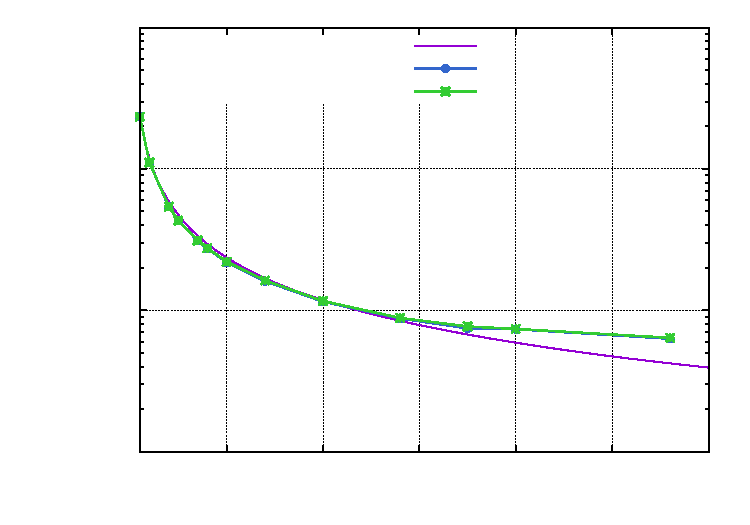
\includegraphics{plot-T-UDN-SM_nogatherInt_selected_500_selected_280}}%
    \gplfronttext
  \end{picture}%
\endgroup
}
%%     \caption{Confronto della scalabilita nelle diverse implementazioni, Ta=181, M=280}
%%   \end{subfigure}
%% \end{figure}
